\documentclass{exam}
\usepackage{../../mypackages}
\usepackage{../../macros}
\usepackage{array}

\title{Interro N°2 - Rattrapage Thaïs. Atome et Réactions Chimiques}
\author{N. Bancel}
\date{4 Décembre 2024}

\begin{document}

\newcolumntype{C}{>{\centering\arraybackslash}m{2cm}}

\textbf{Collège Lycée Suger}
\hfill
\textbf{Physique-Chimie} \\

\textbf{Année 2024-2025}
\hfill
\textbf{3ème Cambridge International} \par

{\let\newpage\relax\maketitle}

\begin{center}
\textbf{\textcolor{red}{Durée : 45 minutes. La calculatrice n'est pas autorisée}} \\
\textbf{\textcolor{red}{Une réponse donnée sans justification sera considérée comme fausse.}} \\
Cette interrogation contient \numquestions\ questions, sur \numpages\ pages et est notée sur 10. 

\end{center}

\section*{Partie 1 : Structure de l'Atome et Propriétés (5 points)}


\begin{questions}
  \question[0.5] Donnez la signification de $A$, $X$, et $Z$ dans la notation symbolique d'un atome.

\begin{figure}[H]
    \centering
    
\includegraphics[width=0.2\linewidth]{interro2_01.jpg}
    \caption{Structure simplifiée d'un atome}
\end{figure} 

  \question[1] Compléter la figure ci-dessous. Il est obligatoire de donner une justification de la méthode en amont (pas besoin de la ré expliquer à chaque fois). Aucun point ne sera attribué si aucune justification n'est apportée.

\begin{table}[H]
  \centering
  \begingroup
  \renewcommand{\arraystretch}{1.5}
  \begin{tabularx}{\textwidth}{|X|C|C|C|C|}
    \hline
    \textbf{Symbole de l’atome} & \textbf{C} & \textbf{Ne} & \textbf{Al} & \textbf{Zn} \\
    \hline
    \textbf{Nom de l’atome} & carbone & néon & aluminium & zinc \\
    \hline
    \textbf{Nombre d’électrons} & 6 & 10 & ... & 30 \\
    \hline
    \textbf{Nombre de nucléons} & 12 & 20 & 27 & ... \\
    \hline
    \textbf{Nombre de protons} & ... & ... & 13 & ... \\
    \hline
    \textbf{Nombre de neutrons} & ... & ... & ... & 35 \\
    \hline
  \end{tabularx}
  \endgroup
\end{table}

\question[0.5] Expliquez pourquoi un atome est neutre électriquement.

\question[1.5] Le chlore est un élément chimique très présent dans la nature. Basé sur les informations ci-dessous, de combien de fois le rayon d'un atome Chlore est-il plus grand que le rayon du noyau de l'atome de Chlore ? Justifier

\begin{center}
\begin{tabular}{SS}
  \toprule
  {Element} & {Rayon (en mètres \si{m})} \\
  \midrule
  {Rayon de l'atome} & {\(79 \times 10^{-12}\)} \\
  {Rayon du noyau de l'atome} & {\(4.6 \times 10^{-15}\)} \\
  \bottomrule
\end{tabular}
\end{center}

\question[0.5] Expliquer la différence entre un atome et une molécule, et donnez un exemple de chaque.

\question[1] Définir ce qu'est un isotope et identifier les isotopes de l'oxygène de numéro atomique Z = 8

\begin{table}[H]
  \centering
  \begingroup
  \renewcommand{\arraystretch}{1.5}
  \begin{tabularx}{0.6\textwidth}{|c|X|X|X|X|X|X|X|}
    \hline
    \textbf{Nombre de protons} & 8 & 4 & 8 & 17 & 35 & 8 & 17 \\
    \hline
    \textbf{Nombre de nucléons} & 17 & 8 & 16 & 37 & 80 & 18 & 35 \\
    \hline
  \end{tabularx}
  \endgroup
\end{table}

\end{questions}

\section*{Partie 2 : Réactions chimiques (5 points)}

\begin{questions}

\question[0.75] Donnez les formules des molécules suivantes :
\begin{itemize}[noitemsep]
  \item Dihydrogène
  \item Dioxyde de carbone
  \item Eau
\end{itemize}



\question[1] La paille de fer (\ce{Fe}) brûle facilement dans l'air (au contact du dioxygène \ce{O2}). Il se forme alors de petites boules d'oxyde magnétique de fer, de formule \ce{Fe3O4}. 
\begin{parts}
  \part[0.25] Quelle est la constitution en atomes de l'oxyde magnétique de fer ? Préciser le nom et le nombre de chaque type d'atomes.
  \part[0.25] Ecrire en toutes lettres la réaction chimique traduisant la transformation entre le fer et le dioxygène de l'air.
  \part[0.5] Ecrire et équilibrer l'équation chimique qui a lieu.
\end{parts}

\question[1]  Adam réalise l'expérience schématisée ci-dessous

\begin{figure}[H]
  \centering
  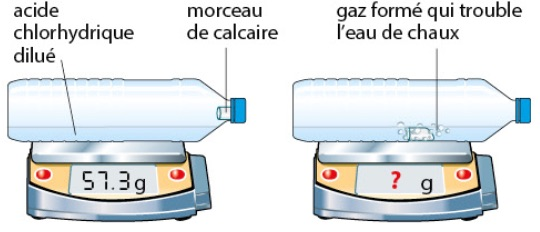
\includegraphics[width=0.6\linewidth]{interro2_03.jpg}
  \caption{Structure simplifiée d'un atome}
\end{figure} 

\begin{parts}
  \part[0.5] Donner le nom des espèces chimiques qui constituent (1) les réactifs (2) les produits. Attention, \textit{"gaz formé qui trouble l'eau de chaud"} n'est pas une espèce chimique.
  \part[0.5] Quelle est la masse des réactifs ? Quelle est la masse des produits (c'est-à-dire : qu'indique la balance de droite ?). Justifier.
\end{parts}


\question[1.5] Les équations chimiques ci-dessous sont-elles équilibrées ? Justifier pourquoi. Si elles ne le sont pas, les équilibrer.
\begin{parts}
  \part[0.5] \ce{C6H12O6 + O2 -> CO2 + H2O}
  \part[0.5] \ce{C + O2 -> CO}
  \part[0.5] \ce{CH4 + O2 -> CO2 + H2O}
\end{parts}

\question[0.75] Quelle est la formule de la réaction chimique ci-dessous ? Est-elle équilibrée ?

\begin{figure}[H]
\centering
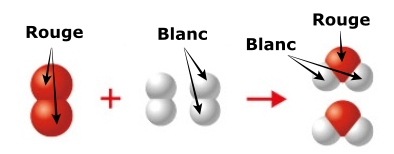
\includegraphics[width=0.6\linewidth]{interro2_04_edited.jpg}
\caption{Réaction chimique}
\end{figure} 


\end{questions}

\section*{Aide au calcul}

Ces calculs (pas tous) peuvent aider à la résolution des exercices :
\begin{itemize}
\item $\frac{79}{4.6} \approx 17.17$
\item $\frac{4.6}{79} \approx 0.05822$
\item $4.6 + 7.9 = 12.5$
\item En considérant $a$ et $b$ des nombres entiers : 
\begin{itemize}
  \item $\frac{10^a}{10^b} = 10^{a-b}$
  \item $10^a \times 10^b = 10^{a+b}$ 
\end{itemize}
\end{itemize}

\end{document}
